% Automaton corresponding to the formulas (Sing(P) and not P
% \subseteq X)

\documentclass{standalone}

\usepackage{pgf}
\usepackage{tikz}
\usepackage{amssymb}
\usepackage{makecell}
\usetikzlibrary{arrows,automata}
\usepackage[latin1]{inputenc}
\begin{document}
%\begin{figure}
% \begin{center}
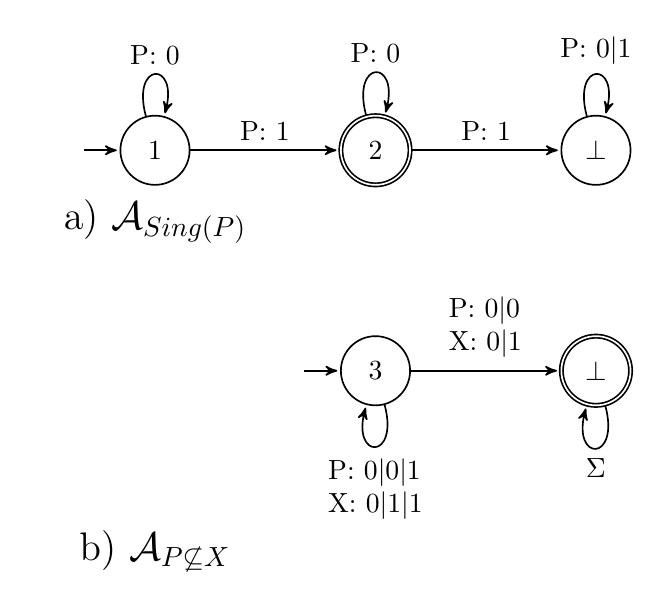
\begin{tikzpicture}[->,>=stealth',shorten >=1pt,auto,node distance=2.8cm,
                    semithick,initial text={}]
  \tikzstyle{every state}=[fill=none,draw=black,text=black]

  \node[initial,state] (A) 				 	{$1$};
  \node[state,accepting] (B) [right of=A]	{$2$};
  \node[state] (C) [right of=B]				{$\bot$};
  
  \node[initial,state] (D) [below of=B] 	{$3$};
  \node[state,accepting] (E) [below of=C]			{$\bot$};
  
  \path (A) edge [loop above] node {P: 0} (A)
  			edge 			  node {P: 1} (B)
  		(B) edge [loop above] node {P: 0} (B)
  		    edge			  node {P: 1} (C)
  		(C) edge [loop above] node {P: 0\textbar 1} (C)
  		
  		(D) edge [loop below] node {\makecell[l]{P: 0\textbar 0\textbar 1\\ X:
  		0\textbar 1\textbar 1}} (D)
  		    edge 			  node {\makecell[l]{P: 0\textbar 0\\ X:
  		    0\textbar 1}} 
  	    (E) (E) edge [loop below] node {$\Sigma$} (E);
  \node [below=4.7cm, align=flush center,text width=3cm] at (A)
        {
            \Large b) $\mathcal{A}_{P \not\subseteq X}$
        };
  \node [below=0.5cm, align=flush center,text width=3cm] at (A)
        {
            \Large a) $\mathcal{A}_{Sing(P)}$
        };
\end{tikzpicture}
% \end{center}
% \caption{Automaton $\mathcal{A}_\phi$ corresponding to the formula $\phi =
% \exists P. (Sing(P) \wedge \neg P \subseteq X)$}
%\end{figure}
\end{document}